% !TEX root = ../main.tex

\section*{How does the engine work?}

First of all, we will explain how is connected the gas circuit, then the ignition sequence and finally, how the combustion starts.

\subsection*{Gas circuit}

The gas circuit begins in the tank, where we can find the gas at the approximate pressure of 60 bars (depending on the tank temperature). A tube joins the tank with the engine chamber, passing through the nozzle and the rocket candy (made of white sugar and potassium nitrate). The rocket candy is connected to an ignitor, when fired, it provides the necessary energy to start the combustion. Before the tubes enter the engine it has to go through an electro-valve that is remotely controlled. To ensure that the valve works, there are two pressure sensors before and after the electro-valve. These sensors will send their readings to the control panel. If the valve fails to open or stops before the tank is full, a pressure difference will be detected thanks to the pressure sensors.

\subsection*{Ignition sequence}

\begin{figure}[h]
  \centering
  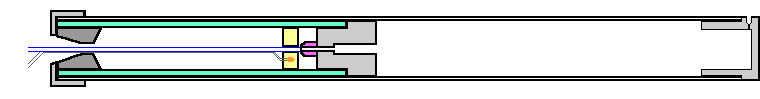
\includegraphics[width=0.8\textwidth,height=2.5cm,keepaspectratio]{seq01.png}
  \caption{Empty motor}
  \label{fig:emptyMotor}
\end{figure}

\begin{figure}[h]
  \centering
  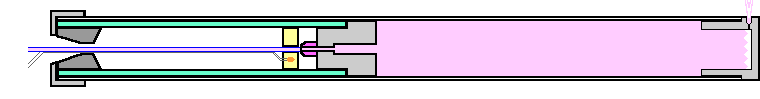
\includegraphics[width=0.8\textwidth,height=2.5cm,keepaspectratio]{seq04.png}
  \caption{Motor filled with $N_2O$ and venting}
  \label{fig:filledMotor}
\end{figure}

The ignition sequence starts by checking the ignitor continuity through the control panel. Once this is done the system is ready to be filled with gas. In order to fill the engine tank with gas, the tank valve must be manually opened and the electro-valve must be opened remotely from the control panel. Once both valves are open the engine tank will fill as seen on Figures \ref{fig:emptyMotor} and \ref{fig:filledMotor}. Once the chamber is full, the electro-valve and the tank valve will be closed.

\begin{figure}[h]
  \centering
  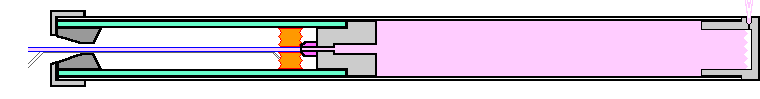
\includegraphics[width=0.8\textwidth,height=2.5cm,keepaspectratio]{seq06.png}
  \caption{The ignitor starts the combustion of the solid grain}
  \label{fig:startSolidBurnMotor}
\end{figure}

Finally, the countdown to the ignition is started through the control panel and the ignitor will be automatically triggered when the countdown reaches 0. The start of the ignitor can be seen on Figure \ref{fig:solidBurningMotor}

\subsection*{Combustion}

\begin{figure}[h]
  \centering
  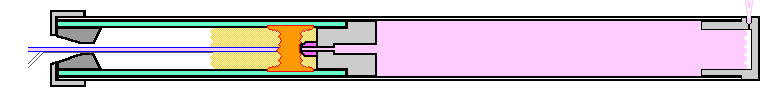
\includegraphics[width=0.8\textwidth,height=2.5cm,keepaspectratio]{seq08.png}
  \caption{The combustion of the solid grain burns the gas tube}
  \label{fig:solidBurningMotor}
\end{figure}

\begin{figure}[h]
  \centering
  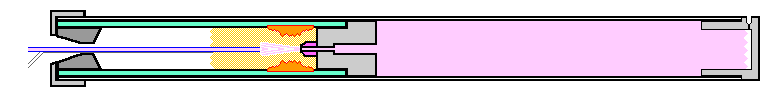
\includegraphics[width=0.8\textwidth,height=2.5cm,keepaspectratio]{seq09.png}
  \caption{The gas leaks through the tube}
  \label{fig:gasLeakingMotor}
\end{figure}

The combustion starts with the spark of the ignitor, which is close to the rocket candy as seen on Figure \ref{fig:solidBurningMotor}. The rocket candy, which is solid fuel, burns rapidly, destroying the walls of the gas tube as seen on Figure \ref{fig:gasLeakingMotor}.

\begin{figure}[H]
  \centering
  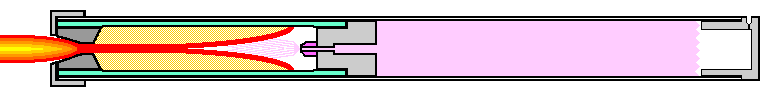
\includegraphics[width=0.8\textwidth,height=2.5cm,keepaspectratio]{seq10.png}
  \caption{The motor is now functioning}
  \label{fig:functioningMotor}
\end{figure}

This damage causes a leak of gas from the tube that burns rapidly too. Finally, this existing flame is able to continue burning the gas of the chamber in conjunction with the polypropylene in the gas chamber, the rocket fully ignited can be seen on Figure \ref{fig:functioningMotor}
